\documentclass[12pt]{article}
\usepackage[brazil]{babel}
\usepackage{graphicx}
\usepackage{mathtools}
\usepackage{float} 
\usepackage{xcolor}


\usepackage{array}
\usepackage{booktabs}



% margenes
\usepackage[a4paper,left=2cm,right=2cm,top=1cm]{geometry}

%opening
\title{\textbf{Modelagem de Escoamentos Turbulentos. \\Lista de Exercícios No. 3}}

\author{Cristian Herledy López Lara}
\date{Junho 2025}

\begin{document}
	
\maketitle


\section*{Questão 1}

Obtenha a equação de transporte para o tensor de Reynolds\\


\textbf{\underline{Desenvolvimento}}

Partindo da equação de conservação de movimimento linear

\begin{equation}
	\frac{\partial U_i}{\partial t} + U_k \frac{\partial U_i}{\partial x_k} = \frac{1}{\rho} \frac{\partial P}{\partial x_i} + \nu \left( \frac{\partial ^ 2 U_i}{\partial x_k \partial x_k}\right) 
\end{equation}

Aplicando o conceito da media de Reynolds $A = \overline{A} + a$ para cada termo:

\begin{equation}
	\frac{\partial U_i}{\partial t} = \frac{\partial \overline{U_i} }{\partial t} + \frac{\partial u_i}{\partial t}
\end{equation}
\begin{equation}
	U_k \frac{\partial U_i}{\partial x_k} = \overline{U_k} \frac{\partial \overline{U_i}}{\partial x_k} + \overline{U_k} \frac{\partial u_i}{\partial x_k} + u_k \frac{\partial \overline{U_i}}{\partial x_k} + u_k \frac{\partial u_i}{\partial x_k} 
\end{equation}
\begin{equation}
	\frac{\partial P}{\partial x_i} = \frac{\partial \overline{P}}{\partial x_i} + \frac{\partial p}{\partial x_i}
\end{equation}
\begin{equation}
	\frac{\partial ^ 2 U_i}{\partial x_k \partial x_k} = \frac{\partial ^ 2 \overline{U_i}}{\partial x_k \partial x_k} +  \frac{\partial ^ 2 u_i}{\partial x_k \partial x_k}
\end{equation}

A equação completa fica então

\begin{equation}
	\frac{\partial \overline{U_i} }{\partial t} + \frac{\partial u_i}{\partial t} + \overline{U_k} \frac{\partial \overline{U_i}}{\partial x_k} + \overline{U_k} \frac{\partial u_i}{\partial x_k} + u_k \frac{\partial \overline{U_i}}{\partial x_k} + u_k \frac{\partial u_i}{\partial x_k} = \frac{1}{\rho} \frac{\partial \overline{P}}{\partial x_i} + \frac{\partial p}{\partial x_i} +  \frac{\partial ^ 2 \overline{U_i}}{\partial x_k \partial x_k} +  \frac{\partial ^ 2 u_i}{\partial x_k \partial x_k}
\end{equation}

Agora tomando só os termos da fluctuação turbulenta

\begin{equation}
	 \frac{\partial u_i}{\partial t} +  \overline{U_k} \frac{\partial u_i}{\partial x_k} + u_k \frac{\partial \overline{U_i}}{\partial x_k} + u_k \frac{\partial u_i}{\partial x_k} = \frac{1}{\rho} \frac{\partial p}{\partial x_i} +  \frac{\partial ^ 2 u_i}{\partial x_k \partial x_k}
\end{equation}

Multiplicando por $u_j$ cada termo da equação

\begin{equation}
	u_j\frac{\partial u_i}{\partial t} = \frac{\partial u_i u_j}{\partial t} - u_i \frac{\partial u_j}{\partial t}
\end{equation}

\begin{equation}
	u_j\overline{U_k} \frac{\partial u_i}{\partial x_k} = \overline{U_k} \frac{\partial u_i u_j}{\partial x_k} - \overline{U_k} u_i \frac{\partial u_i}{\partial x_k}
\end{equation}

\begin{equation}
	u_ju_k \frac{\partial \overline{U_i}}{\partial x_k} 
\end{equation}

\begin{equation}
	u_ju_k \frac{\partial u_i}{\partial x_k} = u_k \frac{\partial u_i u_j}{\partial x_k} - u_iu_k \frac{\partial u_j}{\partial x_k}
\end{equation}

\begin{equation}
	u_j\frac{\partial ^ 2 u_i}{\partial x_k \partial x_k} = \frac{\partial ^ 2 u_i u_j}{\partial x_k \partial x_k} - u_i\frac{\partial ^ 2 u_j}{\partial x_k \partial x_k}
\end{equation}

Escrevendo a equação completa:

\begin{equation}
	\begin{split}
		\frac{\partial u_i u_j}{\partial t} 
		- u_i \frac{\partial u_j}{\partial t} 
		+ \overline{U_k} \frac{\partial u_i u_j}{\partial x_k} 
		- \overline{U_k} u_i \frac{\partial u_i}{\partial x_k} 
		+ u_j u_k \frac{\partial \overline{U_i}}{\partial x_k} 
		+ u_k \frac{\partial u_i u_j}{\partial x_k} 
		- u_i u_k \frac{\partial u_j}{\partial x_k} 
		= \\
		\frac{u_j}{\rho} \frac{\partial p}{\partial x_i} +   \nu\left(  \frac{\partial ^ 2 u_i u_j}{\partial x_k \partial x_k} - u_i\frac{\partial ^ 2 u_j}{\partial x_k \partial x_k}\right) 
	\end{split}
\end{equation}

Da mesma forma, obtemos a equação para a flutuação $u_j$

\begin{equation}
	\begin{split}
		\frac{\partial u_i u_j}{\partial t} 
		- u_j \frac{\partial u_i}{\partial t} 
		+ \overline{U_k} \frac{\partial u_i u_j}{\partial x_k} 
		- \overline{U_k} u_j \frac{\partial u_j}{\partial x_k} 
		+ u_i u_k \frac{\partial \overline{U_i}}{\partial x_k} 
		+ u_k \frac{\partial u_i u_j}{\partial x_k} 
		- u_j u_k \frac{\partial u_j}{\partial x_k} 
		= \\
		\frac{u_i}{\rho} \frac{\partial p}{\partial x_i} + \nu \left(  \frac{\partial ^ 2 u_i u_j}{\partial x_k \partial x_k} - u_j\frac{\partial ^ 2 u_j}{\partial x_k \partial x_k}\right) 
	\end{split}
\end{equation}

Somando a equação 14 da equação 13 obtemos

\begin{equation}
	\begin{split}
		\frac{\partial u_i u_j}{\partial t} 		
		+ \overline{U_k} \frac{\partial u_i u_j}{\partial x_k} + u_j u_k \frac{\partial \overline{U_i}}{\partial x_k} + u_i u_k \frac{\partial \overline{U_i}}{\partial x_k} + \frac{\partial u_i u_j u_k}{\partial x_k}		
		= \\
		\frac{1}{\rho} \left( u_i\frac{\partial p}{\partial x_i} + u_j \frac{\partial p}{\partial x_j} \right) + \nu \left(  u_i\frac{\partial ^ 2  u_j}{\partial x_k \partial x_k} + u_j\frac{\partial ^ 2 u_i}{\partial x_k \partial x_k}\right) 
	\end{split}
\end{equation}

E aplicando os termos da media

\begin{equation}
	\begin{split}
		\frac{\partial \overline{u_i u_j}}{\partial t} 		
		+ \overline{U_k} \frac{\partial \overline{u_i u_j}}{\partial x_k} + \overline{u_j u_k} \frac{\partial \overline{U_i}}{\partial x_k} + \overline{u_i u_k} \frac{\partial \overline{U_i}}{\partial x_k} + \frac{\partial \overline{u_i u_j u_k}}{\partial x_k}		
		= \\
		\frac{1}{\rho} \left( \overline{u_i}\frac{\partial \overline{p}}{\partial x_i} + \overline{u_j} \frac{\partial \overline{p}}{\partial x_j} \right) + \nu \left(  \overline{u_i}\frac{\partial ^ 2  \overline{u_j}}{\partial x_k \partial x_k} + \overline
		{u_j}\frac{\partial ^ 2 \overline{u_i}}{\partial x_k \partial x_k}\right) 
	\end{split}
\end{equation}

\section*{Questão 2}

Simplifique a equação da energia cinética turbulenta $k = (u_i u_i)/2$ para o caso de um
escoamento médio turbulento plenamente desenvolvido em um duto.


\textbf{\underline{Desenvolvimento}}

Agora novamente da equação de transporte do tensor de Reynolds

\begin{equation}
	\begin{split}
		\frac{\partial \overline{u_i u_j}}{\partial t} 		
		+ \overline{U_k} \frac{\partial \overline{u_i u_j}}{\partial x_k} + \overline{u_j u_k} \frac{\partial \overline{U_i}}{\partial x_k} + \overline{u_i u_k} \frac{\partial \overline{U_i}}{\partial x_k} + \frac{\partial \overline{u_i u_j u_k}}{\partial x_k}		
		= \\
		\frac{1}{\rho} \left( \overline{u_i}\frac{\partial \overline{p}}{\partial x_i} + \overline{u_j}  \frac{\partial \overline{p}}{\partial x_j} \right) + \nu \left(  \overline{u_i}\frac{\partial ^ 2  \overline{u_j}}{\partial x_k \partial x_k} + \overline
		{u_j}\frac{\partial ^ 2 \overline{u_i}}{\partial x_k \partial x_k}\right) 
	\end{split}
\end{equation}

Façendo i=j e dividindo por 2 obtemos

\begin{equation}
	\begin{split}
		\frac{\partial k}{\partial t} 		
		+ \overline{U_k} \frac{\partial k}{\partial x_k} + k\frac{\partial \overline{U_i}}{\partial x_k} + k\frac{\partial \overline{U_i}}{\partial x_k} + u_k\frac{\partial k}{\partial x_k}		
		= \frac{1}{\rho} \left( \overline{u_i}\frac{\partial \overline{p}}{\partial x_i}  \right) + \nu \left(  \overline{u_i}\frac{\partial ^ 2  \overline{u_i}}{\partial x_k \partial x_k} \right) 
	\end{split}
\end{equation}

Para escoamento plenamente desenvolvido, a velocidade media na direçao i não muda com relaçao a j, então $\frac{\partial \overline{U_i}}{\partial x_k} = 0$

\begin{equation}
	\begin{split}
		\frac{\partial k}{\partial t} 		
		+ \overline{U_k} \frac{\partial k}{\partial x_k} + u_k\frac{\partial k}{\partial x_k}		
		= \frac{1}{\rho} \left( \overline{u_i}\frac{\partial \overline{p}}{\partial x_i}  \right) + \nu \left(  \overline{u_i}\frac{\partial ^ 2  \overline{u_i}}{\partial x_k \partial x_k} \right) 
	\end{split}
\end{equation}





\begin{table}[h]
	\centering
	\begin{tabular}{|c|c|c|}
		\hline
		Periodo T [s] & U media [m/s] & Desvio padrão [m/s]; \\ \hline
		0 - 0,005   & 8,8854    & 1,0636    \\ \hline
		0 - 0,05   & 8,5692   & 1,1724  \\ \hline
		0 - 0,5    & 8,5342    & 1,2415    \\ \hline
		0 - 5    & 8,5417    & 1,2330   \\ \hline
	\end{tabular}
	\caption{Valores de velocidade media e desvio padrão para diferentes intervalos}
\end{table} 

\begin{figure}[H]
	\centering
	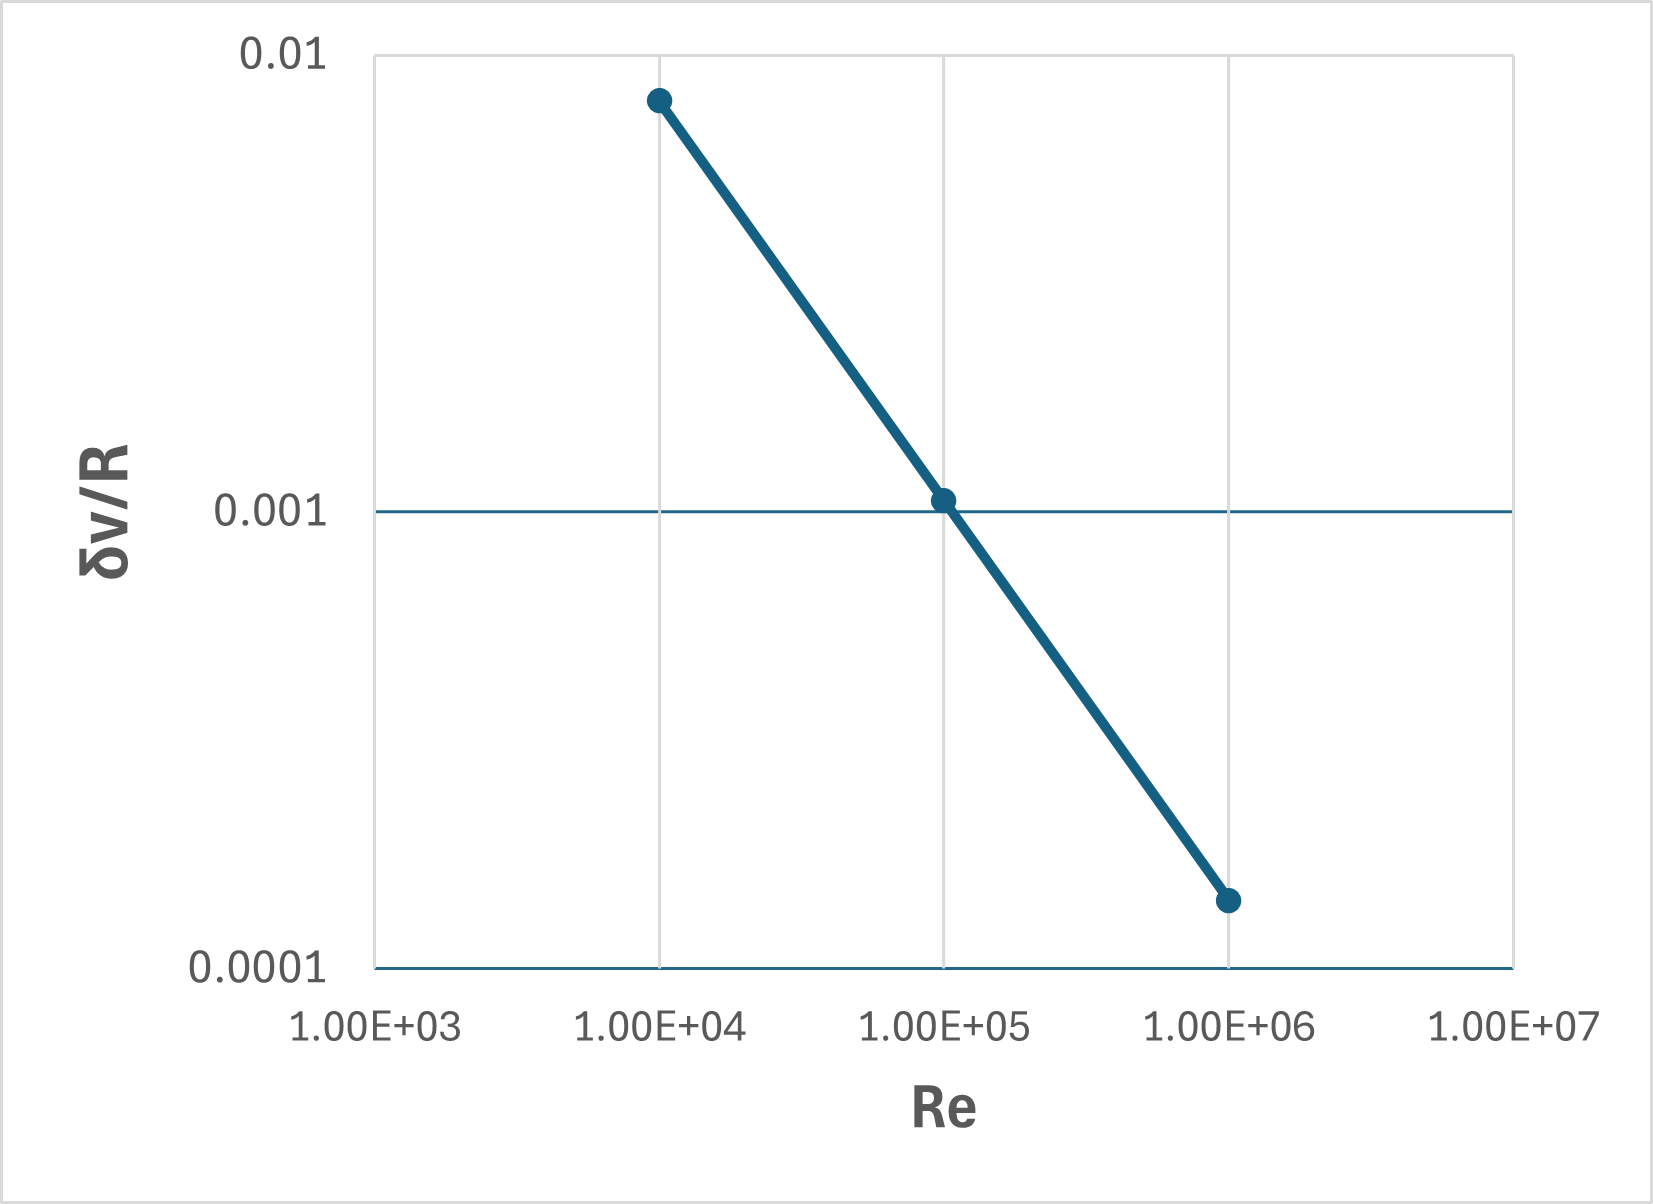
\includegraphics[width=.65\textwidth]{Figures/1.PNG}
	\caption{Velocidade instantanea e velocidade media ate $t=0,05s$}
\end{figure}

O gráfico a seguir mostra a evolução da velocidade média e do desvio padrão. Ambas as grandezas convergem para um valor à medida que o tempo avança. Isso ocorre porque há mais dados para calcular a média da amostra em $t=5s$. As grandes e pequenas escalas terão passado pelo dispositivo de medição um número maior de vezes, o que permite estatísticas turbulentas mais homogêneas e, portanto, a medição do escoamento em regime permanente.

\begin{figure}[H]
	\centering
	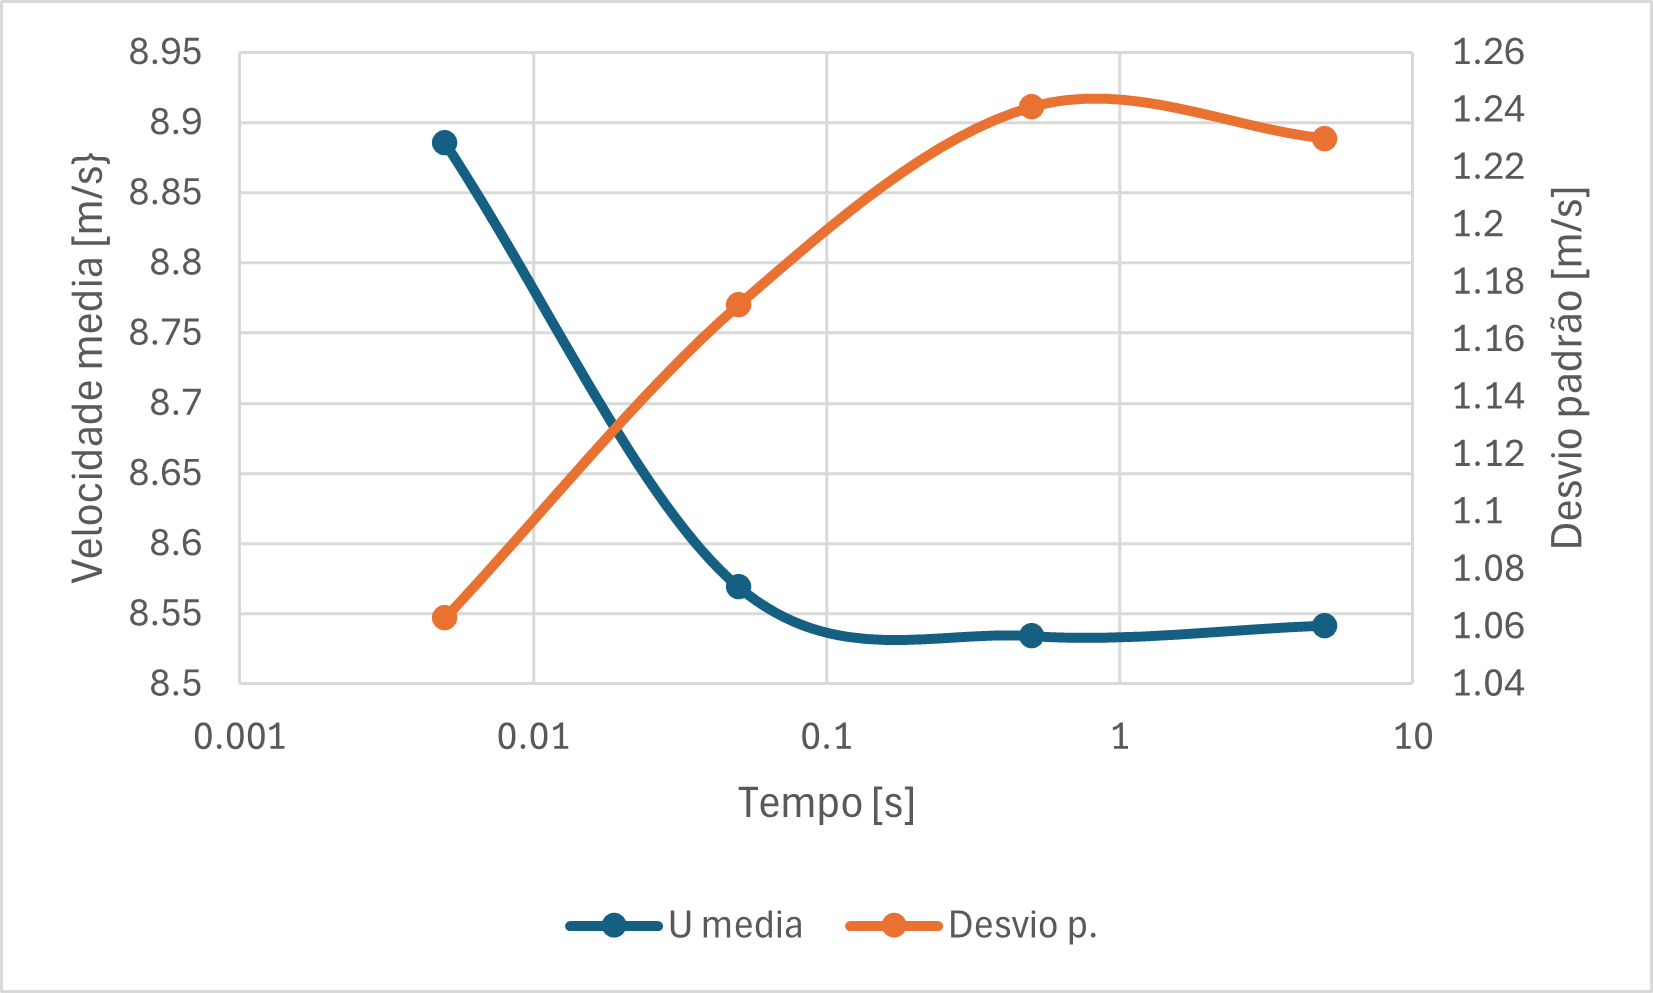
\includegraphics[width=.65\textwidth]{Figures/2.PNG}
	\caption{Velocidade media e desvio padrao nos intervalos de tempo analisados}
\end{figure}


\section*{Questão 2}

A partir dos dados do arquivo Re125.txt:\\
\textbf{i. Determine a energia cinética turbulenta, k, assumindo a condição de isotropia;}\\



A energia cinética turbulenta é calculada com a expressão


\begin{equation}
	k = {\overline{u_i u_i}}/2
\end{equation}
Que para un escoamento isotrópico pode ser escrito como 

\begin{equation}
	k = {\overline{u1u1 + u1u1 + u1u1}}/2 \ = \ \frac{3}{2}\overline{u_1 u_1}^2 \ = \ 2,26 \ \frac{m^2}{s^2}
\end{equation}

\textbf{ii. Faça um gráfico para o coeficiente de correlação temporal e avalie a escala de
comprimento L das grandes escalas;}\\

Para o cálculo de correlação temporal , primeiro é necesario encomtrar o valor da correlação de velocidade no ponto $(r=0)$ dado pela expressão


\begin{equation*}
	\mathbf{R}_{ij}^{(t)}(\mathbf{x}, \boldsymbol{\tau}) = \overline{u_i(\mathbf{x}, t) \, u_j(\mathbf{x}, t')}
\end{equation*}





\begin{thebibliography}{999}
	
	
	\bibitem{Deschamps}
	Cesar Deschamps,
	Escalas da turbulencia Cap 2.
	UFSC Florianopolis, SC,
	Notas de aula,
	2025.
		
	
\end{thebibliography}


\end{document}





